\input{../../university/.preambles/01-semester_work}
\input{../../university/.preambles/10-russian}
\input{../../university/.preambles/20-math}
\input{../../university/.preambles/30-physics}
\begin{document}
\maketitlepage{Факультет электроники и вычислительной техники}{физики}
{Электродинамика}{студент группы Ф-369\\Голубев~А.~В.}
{доцент Грецов~М.~В.}{№2}

\newcommand{\grad}{\mathrm{grad}\,}

\newpage
\emph{Задача №689}: Бесконечно длинная равномерно заряженная прямая с линейной
плотностью заряда \( \varkappa \) в системе, где прямая покоится, перемещается
вдоль своей длины равномерно со скоростью \( v \). На расстоянии \( r \) от неё
находится точечный заряд, движущийся параллельно прямой с той же скоростью. 
Найти электромагнитную силу \( F \), действующую на заряд; скорость \( v \)
произвольна.
\begin{figure}[ht]
    \center
	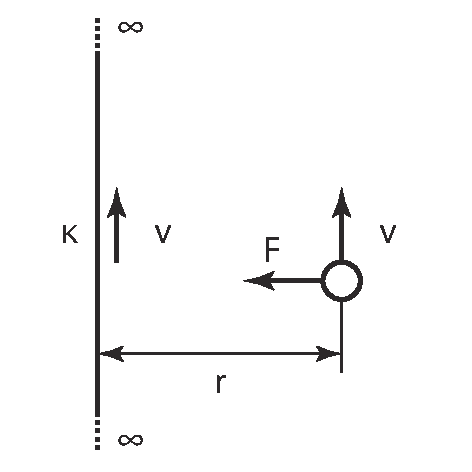
\includegraphics[width=0.4\textwidth]{pdf/01.pdf}
\end{figure}

Запишем уравнение движения заряда в электромагнитном поле:
\[ \frac{d\vec{p}}{dt} = e\vec{E} + \frac{e}{c}\vec{v}\times\vec{H} \]

Стоящие справа выражение носит название \emph{лоренцевой силы}. Первая её 
часть -- сила, с которой действует электрическое поле на заряд, -- не зависит 
от скорости заряда и ориентирована по направлению поля \( \vec{E} \). Вторая 
часть -- сила, оказываемая магнитным полем на заряд, -- пропорциональна скорости 
заряда и направлена перпендикулярно к этой скорости и к направлению магнитного 
поля \( \vec{H} \).

В силу произвольности скорости движения, уравнение можно записать в виде:
\[ 
	\frac{m}{\sqrt{1-\beta^2}}\cdot\frac{d\vec{v}}{dt} = 
	e\vec{E} + \frac{e}{c}\vec{v}\times\vec{H} 
\]

Или представляя \( m\cfrac{d\vec{v}}{dt} = \vec{F} \), перепишем в следующем виде:
\[ \frac{\vec{F}}{\sqrt{1-\beta^2}} = e\vec{E} + \frac{e}{c}\vec{v}\times\vec{H} \]

\newpage

Так как по условию задачи, заряд точечный, то он не будет вносить изменение 
в поле создаваемое движущийся прямой. 

Перейдем в систему связанную с точечным зарядом. 
Магнитное поле не действует на наш заряд, тогда можно положить \( \vec{H} = 0 \), 
и перейти от векторов к скалярам.
\[ F = eE\sqrt{1-\beta^2} \]

Рассмотрим поле, создаваемое бесконечной прямолинейной прямой с линейной плотностью 
\( \varkappa \). Возьмём в качестве поверхности цилиндр с осью, 
совпадающий с прямой, радиусом \( r \) и высотой \( \Delta l \). Тогда поток через 
поверхность по теореме Гаусса:
\[ \Phi_E = \frac{Q}{\varepsilon_0} = \frac{\varkappa\Delta l}{\varepsilon_0} \]

В силу симметрии:
\vspace*{-1em}
\begin{itemize}\itemsep-8pt
	\item[1)] вектор напряженности поля направлен перпендикулярно прямой
	\item[2)] модуль этого вектора в любой точке поверхности цилиндра одинаков
\end{itemize}

Тогда поток напряжённости через эту поверхность можно рассчитать следующим образом:
\[ \Phi_E = \sum_i \Delta S_i E_i = E\sum_i\Delta S_i = ES = E2\pi r\Delta l \]

Учитывая только площадь боковой поверхности цилиндра, так как поток через основания 
цилиндра равен нулю (в следствии направления \( E \) по касательным к ним). 
Приравнивая два полученных выражения для \( \Phi_E \), получаем:
\[ \frac{\varkappa \Delta l}{\varepsilon_0} = E2\pi r\Delta l \]
\[ E = \frac{\varkappa}{2\pi\varepsilon_0 r} \]

Или в системе СГС:
\[ E = \frac{2\varkappa}{r} \]

Подставляя полученную напряженность поля в уравнение для силы получаем:
\[ F = \frac{2e\varkappa}{r}\sqrt{1-\beta^2} \]

\emph{Ответ:}
\[ F = \frac{2e\varkappa}{r}\sqrt{1-\beta^2} \]

\newpage

%------------------------------------------------------------------------------------

\emph{Задача №733}: Исследовать влияние интерференции на излучение 
электро-магнитных волн системой зарядов в следующем примере: два одинаковых
электри-ческих заряда \( e \) движутся равномерно с нерелятивистской скоростью
и с частотой \( \omega \) по круговой орбите радиуса \( a \), оставаясь при
этом на противоположных концах диаметра. Найти поляризацию, угловое 
распределение \( \overline{dl}/d\Omega \) и интенсивность \( \overline{I} \)
излучения. Как изменится интенсивность излучения, если убрать один из зарядов.

\begin{figure}[ht]
    \center
	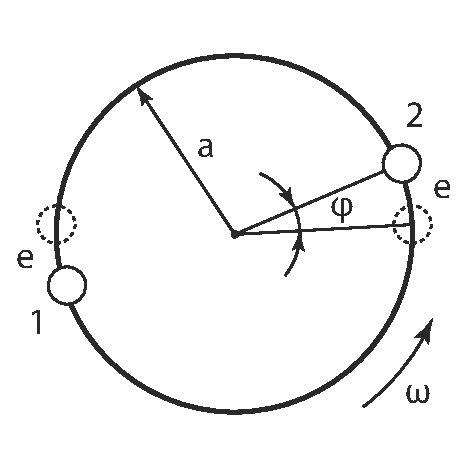
\includegraphics[width=0.4\textwidth]{pdf/02.pdf}
\end{figure}

\emph{Решение:}

Векторный потенциал произвольной системы зарядов с плотностью 
токов \( \vec{j}(\vec{r}, t) \) определяется выражением:
\[ 
	\vec{A}(\vec{r}, t) = \frac{1}{c}\int
	\frac{\vec{j}\left(\vec{r'}, t - \cfrac{|\vec{r}-\vec{r'}|}{c}\right)}
	{|\vec{r} - \vec{r'}|}dV'
\]

Разложим потенциал в ряд по переменной \( (\vec{r}\cdot\vec{r'})/cr \). 
В этом случае первые три члена разложения векторного потенциала имеют вид:
\[
	\vec{A}(\vec{r}, t) = \frac{\dot{\vec{p}}(t')}{cr} + 
	\frac{\ddot{\vec{Q}}(t')}{2c^2 r} + 
	\frac{\dot{\vec{\mu}}(t')\times\vec{n}}{cr}
\]
где \( \vec{n} = \vec{r}/r \) -- единичный радиус вектор точки наблюдения, 
\( t' = t - r/c \) -- время запаздывания, 
\( \vec{p} \) -- дипольный момент системы зарядов,
\( \vec{\mu} \) -- магнитный момент системы токов, а 
\( \vec{Q} \) -- квадрупольный момент, компоненты которого определены 
следующим соотношением:
\[ Q_\alpha = \sum_\beta Q_{\alpha\beta}n_\beta \]

Здесь \( Q_{\alpha\beta} \) -- компоненты тензора квадрупольного момента системы, 
\( n_\beta \) -- компоненты единичного радиус-вектора.

Компоненты тензора квадрупольного момента запишутся в виде:

\[ 
	Q_{\alpha\beta} = \sum_{i=1}^N q_i 
	\left\{ 3x_{\alpha}^{(i)} x_{\beta}^{(i)} - 
	r^{(i)^2}\delta_{\alpha\beta} \right\}
\]

Запишем компоненты тензора квадрупольного момента системы зарядов:
\[ 
	Q_{11} = e\left( 3a^2\cos^2\phi - a^2 \right);\quad
	Q_{12} = e\left( 3a^2\cos\phi\sin\phi \right)
\]
\[ 
	Q_{13} = e\left( 3a^2\cos\phi\cdot 0\right) = 0;\quad
	Q_{21} = e\left( 3a^2\cos\phi\sin\phi \right) 
\]
\[ 
	Q_{22} = e\left( 3a^2\sin^2\phi - a^2 \right);\quad
	Q_{23} = Q_{31} = Q_{32} = 0;
\]
\[ Q_{33} = -ea^2 \]
где \( \phi = \omega t \), \( a \) -- расстояние до заряда.

Найдём квадрупольный момент:
\[ Q_\alpha = \sum_\beta Q_{\alpha\beta}n_\beta \]
\[ 
	Q = 2e \left(\begin{array}{ccc}
		3a^2\cos^2\phi - r^2 & 3a^2\cos\phi\sin\phi & 0 \\
		3a^2\cos\phi\sin\phi & 3a^2\sin^2\phi - a^2 & 0 \\
		0 					 & 0 					& 0
	\end{array}\right) 
	\cdot \left(\begin{array}{c} 
		\vec{e_1} \\
		\vec{e_2} \\
		\vec{e_3} 
	\end{array}\right)
\]

Перемножая строку на столбец, получаем:
\begin{align*}
	& Q = 2e \Big\{
		\left( 3a^2\cos^2\phi - a^2\right)\vec{e_1} + 
		\left( 3a^2\cos\phi\sin\phi \right)\vec{e_2} + 
		0\cdot\vec{e_3} + \\
	&	\left( 3a^2\cos\phi\sin\phi \right)\vec{e_1} +
		\left( 3a^2\sin^2\phi - a^2 \right)\vec{e_2} + 
		0\cdot\vec{e_1} + 0\cdot\vec{e_2} - a^2\vec{e_3}
	\Big\}
\end{align*}

В задаче дипольный и магнитный моменты равны нулю, тогда выражение 
для векторного потенциала запишется в виде: 
\[ 
	\vec{A}(\vec{r}, t) = \frac{\ddot{\vec{Q}}(t')}{2c^2 r}
\]
где точкой обозначено дифференцирование по времени.\\

Найдём первую и вторую производную квадрупольного момента и преобразовав выражения получим:
\[
	\dot{\vec{Q}} = 6ea^2\omega 
	\Big\{
		\left( -\sin{2\omega t'} + \cos{2\omega t'} \right)\vec{e_1} + 
		\left( \cos{2\omega t'} + \sin{2\omega t'} \right)\vec{e_2}
	\Big\}
\]
\[
	\ddot{\vec{Q}} = 12ea^2\omega^2 
	\Big\{
		\left( -\cos{2\omega t'} -\sin{2\omega t'} \right)\vec{e_1} + 
		\left( -\sin{2\omega t'} + \cos{2\omega t'} \right)\vec{e_2}
	\Big\}
\]

В результате векторный потенциал:
\[ 
	\vec{A}(\vec{r}, t) = \frac{6ea^2\omega^2}{c^2r}
	\Big\{
		\left( -\cos{2\omega t'} - \sin{2\omega t'} \right)\vec{e_1} + 
		\left( -\sin{2\omega t'} + \cos{2\omega t'} \right)\vec{e_2}
	\Big\}
\]

Напряженности поля могут быть вычислены по формулам, через векторный потенциал: 
\[ 
	\vec{H}=\frac{1}{c}\dot{\vec{A}}\times\vec{n};\quad
	\vec{E}=\vec{H}\times\vec{n}
\]

Найдём производную векторного потенциала:
\[ 
	\dot{\vec{A}}(\vec{r}, t) = \frac{12ea^2\omega^3}{c^2r}
	\Big\{
		\left(\sin{2\omega t'} - \cos{2\omega t'}\right)\vec{e_1} + 
		\left(-\cos{2\omega t'} - \sin{2\omega t'}\right)\vec{e_2}
	\Big\}
\]

Найдём вектор \( \vec{H} \):
\[ 
	\vec{H} = \frac{12ea^2\omega^3}{c^3r}
	\left(
	\begin{array}{ccc}
		\vec{e_1} & \vec{e_2} & \vec{e_3} \\
		\sin{2\omega t'} - \cos{2\omega t'} & 
		-\cos{2\omega t'} - \sin{2\omega t'} & 0 \\
		0 & 0 & 1
	\end{array}
	\right)
\]

\begin{align*}
	& \vec{H} = \frac{12ea^2\omega^3}{c^3r} \Big\{
		-\vec{e_1}\left( \cos{2\omega t'} - \sin{2\omega t'} \right)
		-\vec{e_2}\left( \sin{2\omega t'} - \cos{2\omega t'} \right)
	\Big\}
\end{align*}

Теперь найдём вектор \( \vec{E} \):
\[ 
	\vec{E} = \frac{12ea^2\omega^3}{c^3r}
	\left(
	\begin{array}{ccc}
		\vec{e_1} & \vec{e_2} & \vec{e_3} \\
		\left( \cos{2\omega t'} - \sin{2\omega t'} \right) & 
		\left( \sin{2\omega t'} - \cos{2\omega t'} \right) & 0 \\
		0 & 0 & 1
	\end{array}
	\right)
\]

\begin{align*}
	& \vec{E} = \frac{12ea^2\omega^3}{c^3r} \Big\{
		\vec{e_1}\left( \sin{2\omega t'} - \cos{2\omega t'} \right)
		-\vec{e_2}\left( \cos{2\omega t'} - \sin{2\omega t'} \right)
	\Big\}
\end{align*}

Найдём вектор Пойнтинга:
\[ |\vec{\Pi}| = \frac{c}{4\pi}\vec{E}\times\vec{H} \]

Подставляя значения для векторов \( \vec{E} \) и \( \vec{H} \) получаем:
\[ |\vec{\Pi}| = \frac{72e^2a^4\omega^6}{\pi c^5 r^2} \]

Средняя интенсивность излучения:
\[ 
	<I> = < \oint \vec{\Pi}\cdot\vec{dS} > = 
	<|\vec{\Pi}|\pi r^2> = \frac{72e^2a^4\omega^6}{c^5}
\]

Угловое распределение интенсивности:
\[ 
	<\frac{dI}{d\Omega}> = <|\vec{\Pi}|r^2> = 
	\frac{72e^2a^4\omega^6}{\pi c^5} 
\]

Если убрать один из зарядов, то интенсивность излучения возрастёт по порядку 
величины \( (\lambda/a)^2 \) раз, то есть значительно, так как выполняется 
условие \( a/\lambda \ll 1 \).\\

\emph{Ответ:}
\[ <I> = \frac{72e^2a^4\omega^6}{c^5} \]
\[ <\frac{dI}{d\Omega}> = \frac{72e^2a^4\omega^6}{\pi c^5} \]

\newpage

%------------------------------------------------------------------------------------

\emph{Задача №776}: Заряд \( e \) движется по окружности радиуса \( a \)
со скоростью \( v = \beta c \). Найти спектральное разложение интенсивности излучения
\( dI_n / d\Omega \) в данном направлении.

\begin{figure}[ht]
    \center
	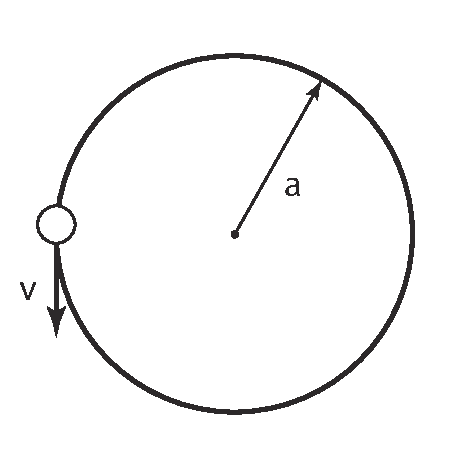
\includegraphics[width=0.4\textwidth]{pdf/03.pdf}
\end{figure}

\[
    \der{I}{\Omega} = |\vec{\varPi}|\cdot r^2,
\]
где \( \vec{\varPi} \) -- вектор Пойнтинга. Считая в волновой зоне участок 
фронта волны вблизи точки наблюдения плоским, можем записать, что
\[
    \varPi = \frac{c}{\mu_0}B^2.
\]
Усреднив по времени, получим
\[
    \der{\bar{I}}{\Omega} = \frac{cr^2}{\mu_0}\bar{B^2}.
\]
Разложим индукцию магнитного поля в ряд Фурье по частоте обращения заряда \( \omega = \beta c/a \):
\[
    B = \sum_{n=-\infty}^{\infty}B_n e^{in\omega t},\text{ где }
    B_n = \frac{1}{T}\int\limits_0^T Be^{-in\omega t}\,dt.
\]
Отсюда
\[
    \bar{B^2} = \sum_{n=-\infty}^{\infty}B_nB_{-n} = 2\sum_{n=1}^\infty |B_n|^2.
\]
Таким образом, для интенсивности имеем
\[
    \der{\bar{I}}{\Omega} = \frac{2cr^2}{\mu_0}\sum_{n=1}^\infty |B_n|^2,
\]
а для отдельных гармоник
\[
    \der{\bar{I}_n}{\Omega} = \frac{2cr^2}{\mu_0}|B_n|^2,
\]
Индукцию \( B_n \) \( n \)-ой гармоники будем искать при помощи векторного потенциала \( \vec{A}_n \):
\[
    \vec{B_n} = rot\vec{A}_n = i\vec{k}\times\vec{A}_n,
\]
где \( k = n\omega/c = n\beta/a \) и \( \vec{k}\parallel\vec{r} \).
Теперь определим разложение в ряд Фурье векторного потенциала. Сам потенциал для точечной частицы, имеющей заряд \( e \) и движущейся со скоростью \( \vec{v} \) имеет вид
\[
    \vec{A} = \frac{\mu_0}{4\pi}\frac{e\vec{v}(t-\frac{R}{c})}{R(t-\frac{R}{c})},
\]
а коэффициенты его разложения в ряд Фурье определяются следующим образом:
\[
    \vec{A}_n = \frac{\mu_0 e}{4\pi T}\int\limits_0^T \frac{\vec{v}(t-\frac{R}{c})}{R(t-\frac{R}{c})}e^{-in\omega t}\,dt.
\]
Не допуская большой ошибки, можно считать, что в знаменателе \( R = r \). Также
учтём, что \( \vec{v}(t-\frac{R}{c})\,dt = d\vec{r'}(t-\frac{R}{c}) \):
\[
    \vec{A}_n = \frac{\mu_0 e}{4\pi rT}\oint e^{-in\omega t - i\vec{k}\cdot\vec{R}}\,d\vec{r'} = \frac{\mu_0 e}{4\pi rT}\oint e^{-in\omega t - i\vec{k}\cdot(\vec{r} - \vec{r'})}\,d\vec{r'} = \frac{\mu_0 e}{4\pi rT}e^{-ikr}\oint e^{-in\omega t+i\vec{k}\cdot\vec{r'}}\,d\vec{r'}.
\]
Введём прямоугольную декартову систему координат \( Oxyz \) с началом в центре окружности, по которой вращается заряд, так, чтобы ось \( Oz \) была перпендикулярна плоскости кольца, а \( \vec{r} \) лежал в плоскости \( Oyz \). Обозначим угол между осью \( Oz \) и \( \vec{r} \) \( \theta \), а угол между осью \( Ox \) и \( \vec{r'} \) \( \phi \). Тогда
\[
    \vec{k}\cdot\vec{r'} = ka\sin\theta\sin\phi = n\beta\sin\theta\sin\phi.
\]
Найдём проекции \( \vec{A}_n \)  на эти оси. Очевидно, что \( A_{nz} = 0 \). Две другие проекции определяют следующим образом
\[
    A_{nx} = -\frac{\mu_0 e}{4\pi rT}e^{-ikr}\int\limits_0^{2\pi} e^{-in(\phi-\beta\sin\theta\sin\phi)}a\sin\phi\,d\phi = -i\frac{2\pi\mu_0 ea}{4\pi rT}e^{-ikr}J_n'(n\beta\sin\theta),
\]
\[
    A_{ny} = -\frac{\mu_0 e}{4\pi rT}e^{-ikr}\int\limits_0^{2\pi} e^{-in(\phi-\beta\sin\theta\sin\phi)}a\cos\phi\,d\phi = \frac{2\pi\mu_0 ea}{4\pi rT\beta\sin\theta}e^{-ikr}J_n(n\beta\sin\theta).
\]
Вернёмся теперь к \( |B_n| \):
\[
    |B_n|^2 = |\vec{k}\times\vec{A}_n|^2 = k^2(A_{nx}^2 + A_{ny}^2\cos^2\theta).
\]
Подставляя последнее равенство в выражение для интенсивности, получим:
\[
    \der{\bar{I}_n}{\Omega} = \frac{\mu_0e^2c^3\beta^2}{8\pi^2a^2}(\ctan^2\theta J_n^2(n\beta\sin\theta) + \beta^2 {J_n'}^2(n\beta\sin\theta)).
\]

Сделаем проверку размерности:
\[
    \left[\der{\bar{I}_n}{\Omega}\right] = \frac{\frac{\text{Гн}}{\text{м}}\cdot\text{Кл}^2\cdot\frac{\text{м}^3}{\text{с}^3}}{\text{м}^2} =  \frac{\text{Дж}}{\text{с}}.
\]

\emph{Ответ:}
\[
    \der{\bar{I}_n}{\Omega} = \frac{\mu_0e^2c^3\beta^2}{8\pi^2a^2}(\ctan^2\theta J_n^2(n\beta\sin\theta) + \beta^2 {J_n'}^2(n\beta\sin\theta)).
\]
\end{document}